\documentclass[11pt]{article}
\usepackage[a4paper,margin=2.5cm]{geometry}
\usepackage{amsmath}
\usepackage{enumitem}
\usepackage{hyperref}
\usepackage{amssymb}
\usepackage{graphicx}
\usepackage{tikz}
\usepackage{amsthm} % for proof environment
\usepackage{bm}

\newif\ifshowanswers
% \showanswerstrue % Uncomment to include answers / Comment to hide answers

\begin{document}

\section*{Exercise 1: Maximum likelihood estimation for a Gaussian}

The Gaussian pdf parametrised by mean $\mu$ and standard deviation $\sigma$ is given by
\[
p(x; \theta) = \frac{1}{\sqrt{2\pi \sigma^2}} \exp\left[ -\frac{(x - \mu)^2}{2\sigma^2} \right], \quad \theta = (\mu, \sigma).
\]

\noindent
Assume we have iid data $\mathcal{D} = \{x_1, \dots, x_n\}$ drawn from this distribution.
\begin{enumerate}[label=(\alph*)]
  \item Write down the likelihood function $L(\theta)$.
  \item Write down the log-likelihood function $\ell(\theta) = \log L(\theta)$.
  \item Find the maximum likelihood estimates (MLEs) of $\mu$ and $\sigma$.
\end{enumerate}


\ifshowanswers
  \paragraph{Solution.}

\subsection*{(a) Likelihood function}

Given iid data $\mathcal{D} = \{x_1, \dots, x_n\}$, the likelihood function $L(\theta)$ is:
\begin{align}
L(\theta) &= \prod_{i=1}^n p(x_i; \theta) \\
&= \prod_{i=1}^n \frac{1}{\sqrt{2\pi \sigma^2}} \exp\left[ -\frac{(x_i - \mu)^2}{2\sigma^2} \right] \\
&= \frac{1}{(2\pi \sigma^2)^{n/2}} \exp\left[ -\frac{1}{2\sigma^2} \sum_{i=1}^n (x_i - \mu)^2 \right].
\end{align}

\subsection*{(b) Log-likelihood function}

Taking the logarithm of the likelihood function:
\[
\ell(\theta) = -\frac{n}{2} \log(2\pi \sigma^2) - \frac{1}{2\sigma^2} \sum_{i=1}^n (x_i - \mu)^2.
\]

\subsection*{(c) Maximum likelihood estimates}

Define $v = \sigma^2$ for convenience. The log-likelihood becomes:
\[
J(\mu, v) = -\frac{n}{2} \log(2\pi v) - \frac{1}{2v} \sum_{i=1}^n (x_i - \mu)^2.
\]

Taking partial derivatives:
\begin{align}
\frac{\partial J}{\partial \mu} &= \frac{1}{v} \sum_{i=1}^n (x_i - \mu) = \frac{1}{v} \left( \sum_{i=1}^n x_i - n\mu \right), \\
\frac{\partial J}{\partial v} &= -\frac{n}{2v} + \frac{1}{2v^2} \sum_{i=1}^n (x_i - \mu)^2.
\end{align}

Setting derivatives to zero:
\[
\sum_{i=1}^n (x_i - \mu) = 0 \quad \Rightarrow \quad \hat{\mu} = \frac{1}{n} \sum_{i=1}^n x_i,
\]
\[
-\frac{n}{2v} + \frac{1}{2v^2} \sum_{i=1}^n (x_i - \hat{\mu})^2 = 0 \quad \Rightarrow \quad \hat{v} = \frac{1}{n} \sum_{i=1}^n (x_i - \hat{\mu})^2.
\]

So the MLEs are:
\begin{align}
\hat{\mu} &= \frac{1}{n} \sum_{i=1}^n x_i, \\
\hat{\sigma} &= \sqrt{ \frac{1}{n} \sum_{i=1}^n (x_i - \hat{\mu})^2 }.
\end{align}
\fi

\section*{Exercise 2: Cancer-asbestos-smoking example: MLE}

The cancer-asbestos-smoking example illustrates a causal structure where,
the variables are: a (asbestos exposure), s (smoking), and c (cancer).
The model assumes that both asbestos exposure and smoking independently contribute to the risk of developing cancer, while they are independent of each other.

\begin{figure}[h]
\centering
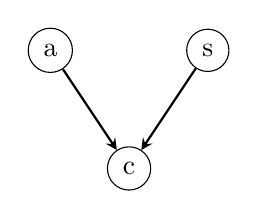
\begin{tikzpicture}[node distance=2cm, every node/.style={draw,circle}]
    \node (a) {a};
    \node (s) [right of=a] {s};
    \node (c) [below of=a, node distance=1.5cm, xshift=1cm] {c};

    \draw [->, thick, >=stealth] (a) -- (c);
    \draw [->, thick, >=stealth] (s) -- (c);
\end{tikzpicture}
\caption{Graphical model for the cancer-asbestos-smoking example.}
\end{figure}

\noindent
The distributions of $a$ and $s$ are Bernoulli distributions with success probabilities $\theta_a$ and $\theta_s$, respectively:
\[
p(a; \theta_a) = \theta_a^a (1 - \theta_a)^{1 - a}, \quad p(s; \theta_s) = \theta_s^s (1 - \theta_s)^{1 - s}.
\]

\noindent
The distribution of $c$ given the parents is parametrised as follows:

\[
\begin{array}{cc|c}
  a & s & p(c = 1 \mid a, s) \\
\hline
0 & 0 & \theta_c^1 \\
1 & 0 & \theta_c^2 \\
0 & 1 & \theta_c^3 \\
1 & 1 & \theta_c^4 \\
\end{array}
\]

\noindent
The free parameters of the model are $\bm{\theta} = (\theta_a, \theta_s, \theta_c^1, \theta_c^2, \theta_c^3, \theta_c^4)$. Assume we observe the following iid data (each row is a data point):

\[
\begin{array}{cc|c}
a & s & c \\
\hline
0 & 1 & 1 \\
0 & 0 & 0 \\
1 & 0 & 1 \\
0 & 0 & 0 \\
0 & 1 & 0 \\
\end{array}
\]

\noindent
Determine the maximum-likelihood estimates (MLEs) of the parameters $\bm{\theta}$.

\ifshowanswers
\paragraph{Solution.}
We first determine the maximum-likelihood estimates of $\theta_a$ and $\theta_s$
The MLE of $\theta_a$ is the empirical frequency of $a=1$:
\[
\hat{\theta}_a = \frac{1}{5}.
\]

Similarly, the MLE of $\theta_s$ is:
\[
\hat{\theta}_s = \frac{2}{5}.
\]

\noindent
We then determine the maximum-likelihood estimates of $\theta_c^1, \ldots, \theta_c^4$.
We count the occurrences of each parent configuration $(a, s)$ and how often $c=1$ happens given each configuration.

\[
\begin{array}{cccc|l}
a & s & \text{Count} & \text{\# with } c=1 & \hat{\theta}_c^{\cdot} \\
\hline
0 & 0 & 2 & 0 & \hat{\theta}_c^1 = 0/2 = 0 \\
1 & 0 & 1 & 1 & \hat{\theta}_c^2 = 1/1 = 1 \\
0 & 1 & 2 & 1 & \hat{\theta}_c^3 = 1/2 = 0.5 \\
1 & 1 & 0 & - & \hat{\theta}_c^4 \text{ undefined} \\
\end{array}
\]

Notes:
\begin{itemize}
  \item $\hat{\theta}_c^4$ is undefined because the parent configuration $(a=1, s=1)$ does not appear in the dataset.
  \item Some estimates are $0$ or $1$, indicating overfitting — a common issue with MLE when data is sparse.
\end{itemize}

\fi

\section*{Exercise 3: Cancer-asbestos-smoking example: MAP}

Now assume a prior distribution over the parameters $\bm{\theta}$, given by
\[
  p(\theta) = \mathcal{U}(0, 1), \quad \text{for each } \theta \in \bm{\theta}.
\]

\noindent
Determine the maximum a posteriori (MAP) estimates of the parameters $\bm{\theta}$ given the same data as in Exercise 2.
\ifshowanswers
  \paragraph{Solution.}
  The MAP estimate maximises the posterior distribution:
  \[
    \hat{\bm{\theta}}_{\text{MAP}} = \arg\max_{\bm{\theta}} p(\bm{\theta} \mid \mathcal{D}) = \arg\max_{\bm{\theta}} p(\mathcal{D} \mid \bm{\theta}) p(\bm{\theta}).
  \]
  Since the prior is uniform, it does not affect the maximisation, and we can focus on the likelihood:
  \[
    \hat{\bm{\theta}}_{\text{MAP}} = \arg\max_{\bm{\theta}} p(\mathcal{D} \mid \bm{\theta}).
  \]
  The MLEs from Exercise 2 are also the MAP estimates in this case, as the uniform prior does not change the maximisation:
  \begin{align*}
    \hat{\theta}_a &= \frac{1}{5}, \\
    \hat{\theta}_s &= \frac{2}{5}, \\
    \hat{\theta}_c^1 &= 0, \\
    \hat{\theta}_c^2 &= 1, \\
    \hat{\theta}_c^3 &= 0.5, \\
    \hat{\theta}_c^4 &\text{ undefined}.
  \end{align*}
\fi

\section*{Exercise 4: Cancer-asbestos-smoking example: Posterior Distribution}

As above, we assume a prior distribution over the parameters $\bm{\theta}$, given by
\[
  p(\theta) = \mathcal{U}(0, 1), \quad \text{for each } \theta \in \bm{\theta}.
\]

\noindent
and assume we observe the same iid data as in Exercise 2.
\noindent
Determine the posterior distribution $p(\bm{\theta} \mid \mathcal{D})$.


\paragraph{Hint.}
Beta and Bernoulli distributions are conjugate, meaning that if the prior is a Beta distribution and the likelihood is a Bernoulli distribution, the posterior will also be a Beta distribution.
Let \(\theta \in [0, 1]\) be a parameter with prior:

\[
\theta \sim \text{Beta}(\alpha_0, \beta_0)
\]

\noindent
Let \(x_1, x_2, \dots, x_n \sim \text{Bernoulli}(\theta)\) be independent observations.
Define:
\[
n_1 = \sum_{i=1}^n x_i \quad \text{(number of ones)}, \qquad n_0 = n - n_1 \quad \text{(number of zeros)}
\]

\noindent
Then the posterior distribution is:

\[
\boxed{
\theta \mid x_{1:n} \sim \text{Beta}(\alpha_0 + n_1, \, \beta_0 + n_0)
}
\]

\noindent
The posterior mean is:

\[
\boxed{
\mathbb{E}[\theta \mid x_{1:n}] = \frac{\alpha_0 + n_1}{\alpha_0 + \beta_0 + n}
}
\]

\noindent
\textbf{Special Case: Uniform Prior.}
If the prior is uniform, i.e., \(\theta \sim \text{Beta}(1, 1)\), then:

\[
\theta \mid x_{1:n} \sim \text{Beta}(1 + n_1, \, 1 + n_0)
\]

\noindent
and the posterior mean becomes:

\[
\boxed{
\mathbb{E}[\theta \mid x_{1:n}] = \frac{1 + n_1}{2 + n}
}
\]

\ifshowanswers
  \paragraph{Solution.}

We are given a directed graphical model with binary variables \(a\), \(s\), and \(c\), where:

\begin{itemize}
  \item \(a, s \sim \text{Bernoulli}(\theta_a), \text{Bernoulli}(\theta_s)\)
  \item \(c \mid a, s \sim \text{Bernoulli}(\theta_c^{(a,s)})\)
\end{itemize}

We assume a uniform prior over all parameters which equivalently is a Beta distribution with parameters (1, 1):
\[
\theta_a, \theta_s, \theta_c^1, \theta_c^2, \theta_c^3, \theta_c^4 \sim \text{Beta}(1,1)
\]

We are given 5 data points:

\[
\begin{array}{ccc}
a & s & c \\
\hline
0 & 1 & 1 \\
0 & 0 & 0 \\
1 & 0 & 1 \\
0 & 0 & 0 \\
0 & 1 & 0 \\
\end{array}
\]

\subsection*{Posterior of \(\theta_a\)}

Let \(n = 5\), and \(k = \#\{a=1\} = 1\), then:

\[
\theta_a \mid D \sim \text{Beta}(1 + 1, 1 + 4) = \text{Beta}(2, 5)
\]

\[
\mathbb{E}[\theta_a \mid D] = \frac{2}{2 + 5} = \frac{2}{7}
\]

\subsection*{Posterior of \(\theta_s\)}

Number of \(s = 1\) entries: \(k = 2\), \(n = 5\)

\[
\theta_s \mid D \sim \text{Beta}(1 + 2, 1 + 3) = \text{Beta}(3, 4)
\]

\[
\mathbb{E}[\theta_s \mid D] = \frac{3}{3 + 4} = \frac{3}{7}
\]

\subsection*{Posterior of \(\theta_c^{(a,s)}\)}

Let \(\theta_c^{(a,s)}\) denote the probability \(\mathbb{P}(c = 1 \mid a, s)\). We compute counts for each configuration:

\begin{itemize}
  \item \((a=0, s=0)\): occurs 2 times, \(c=1\) occurs 0 times.

  \[
  \theta_c^1 \sim \text{Beta}(1 + 0, 1 + 2) = \text{Beta}(1, 3), \quad \mathbb{E}[\theta_c^1] = \frac{1}{4}
  \]

  \item \((a=1, s=0)\): occurs 1 time, \(c=1\) occurs 1 time.

  \[
  \theta_c^2 \sim \text{Beta}(1 + 1, 1 + 0) = \text{Beta}(2, 1), \quad \mathbb{E}[\theta_c^2] = \frac{2}{3}
  \]

  \item \((a=0, s=1)\): occurs 2 times, \(c=1\) occurs 1 time.

  \[
  \theta_c^3 \sim \text{Beta}(1 + 1, 1 + 1) = \text{Beta}(2, 2), \quad \mathbb{E}[\theta_c^3] = \frac{1}{2}
  \]

  \item \((a=1, s=1)\): occurs 0 times

  \[
  \theta_c^4 \sim \text{Beta}(1, 1), \quad \mathbb{E}[\theta_c^4] = \frac{1}{2} \quad \text{(same as prior)}
  \]
\end{itemize}

\subsection*{Summary of Posterior Means}

\[
\begin{array}{ll}
\mathbb{E}[\theta_a \mid D] &= \frac{2}{7} \\
\mathbb{E}[\theta_s \mid D] &= \frac{3}{7} \\
\mathbb{E}[\theta_c^1 \mid D] &= \frac{1}{4} \\
\mathbb{E}[\theta_c^2 \mid D] &= \frac{2}{3} \\
\mathbb{E}[\theta_c^3 \mid D] &= \frac{1}{2} \\
\mathbb{E}[\theta_c^4 \mid D] &= \frac{1}{2} \quad \text{(uninformed)} \\
\end{array}
\]


\fi

\section*{Exercise 5: Comparison of MLE and expected value of the posterior}

In the previous exercises, we computed the maximum likelihood estimates (MLEs) and the expected values of the posterior distributions for the parameters of the cancer-asbestos-smoking example. Compare the MLEs and the expected values of the posterior distributions for each parameter. What is the conclusion?

  \ifshowanswers
    \paragraph{Solution.}
\[
  \begin{array}{l|c|c}
    \text{Parameter} & \text{MLE / MAP} & \text{Posterior Mean (Beta)} \\
    \hline
    \theta_a & \frac{1}{5} = 0.2 & \frac{2}{7} \approx 0.286 \\
    \theta_s & \frac{2}{5} = 0.4 & \frac{3}{7} \approx 0.429 \\
    \theta_c^1 & 0 & \frac{1}{4} = 0.25 \\
    \theta_c^2 & 1 & \frac{2}{3} \approx 0.667 \\
    \theta_c^3 & 0.5 & 0.5 \\
    \theta_c^4 & \text{undefined} & 0.5 \\
    \hline
  \end{array}
\]

The conclusion is that the MLEs are often more extreme (0 or 1) compared to the expected values of the posterior distributions, which tend to be more moderate. This is particularly evident for \(\theta_c^1\) and \(\theta_c^2\), where the MLEs are 0 and 1, respectively, while the posterior means are more balanced. The uniform prior in the posterior calculation helps to regularise the estimates, preventing overfitting to the data.

\fi


\end{document}
